\documentclass{beamer}

\mode<presentation> {

\usetheme{Copenhagen}
\usecolortheme{seagull}
}

\usepackage{graphicx}
\DeclareGraphicsExtensions{.pdf,.png,.jpg}
\usepackage{booktabs} % Allows the use of \toprule, \midrule and \bottomrule in tables
\usepackage{mathtools}
\usepackage{multirow}
\usepackage{color, colortbl}
\usepackage{minted}

%----------------------------------------------------------------------------------------
%	TITLE PAGE
%----------------------------------------------------------------------------------------

\title[Test]{Test}

\author{Rasmus Guldborg Pedersen}

\date{June 2015}

\begin{document}

\begin{frame}
\titlepage
\end{frame}

\begin{frame}
\frametitle{Overview}
\tableofcontents
\end{frame}




\section{Q 1.3: Review and SMART}
\begin{frame}
    \frametitle{Review Types}
    \begin{itemize}
        \item Informal
            % Done often. The review is not documented.
        \item Formal
    \end{itemize}
\end{frame}

\begin{frame}
    \frametitle{Formal Review}
    \begin{enumerate}
        \item Planning
            \begin{itemize}
                \item Date
                \item Place
                \item Entry criteria
                    % No obvious defects
                \item Exit criteria
            \end{itemize}
        \item Kick-off meeting (optional)
            % Objectives are explained
            % Documents are handed out, including support documents
        \item Preparation
            % Reviewed individually
            % Defects logged
            % Checking rate. Number of pages per hour (5-10 pages common)
        \item Review meeting
            \begin{itemize}
                \item Logging phase % Defects are logged, numbered and rated
                \item Discussion phase % Any defects that needs discussion
                \item Decision phase % Is another review required?
            \end{itemize}
        \item Rework
            % The item under review is improved according to the found defects
        \item Follow-up
            % Moderator insures the author has worked out the defects
    \end{enumerate}
\end{frame}

\begin{frame}
    \frametitle{Review Roles}
    \begin{itemize}
        \item Author
            % Rework the item under review
        \item Moderator
            % Leads the review process
            % Plan meetings
        \item Scribe
            % Log defects
            % Record
        \item Reviewers
            % Find defects
            % Can have a special focus area
        \item Manager
            % Allocates resources for reviews
            % Ultimate decision power
    \end{itemize}
\end{frame}

\begin{frame}
    \frametitle{SMART}
    \begin{itemize}
        \item \textbf{S}pecific
        \item \textbf{M}easurable
        \item \textbf{A}cceptable % attainable
        \item \textbf{R}ealistic % relevant
        \item \textbf{T}raceable % timely, tangible
    \end{itemize}
\end{frame}

\begin{frame}
    \frametitle{W Model}
    \begin{center}
        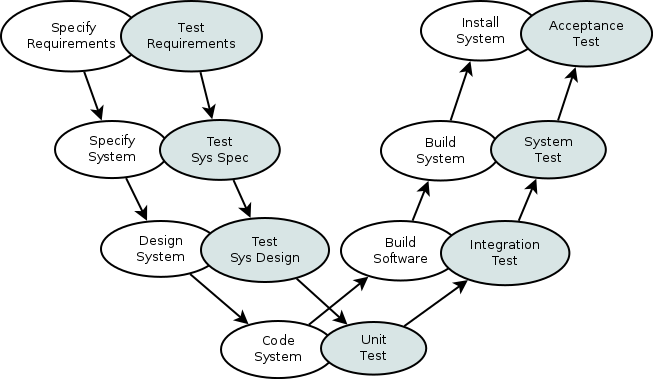
\includegraphics[scale=0.4]{w_model.png}
    \end{center}
\end{frame}


%------------------------------------------------

\begin{frame}
    \frametitle{The End}

    %\Huge{\centerline{The End}}
    \begin{quote}
        ``Testing shows the presence, not the absence of bugs.''
        \raggedleft{--- Edsger W. Dijkstra}
    \end{quote}
\end{frame}

%----------------------------------------------------------------------------------------

\end{document}

